\documentclass[12pt, titlepage]{article}
\usepackage[utf8]{inputenc}
\usepackage{pgfplots}
\usepackage{amsmath}
\usepackage{amsfonts}
\usepackage{amssymb}
\usepackage{multicol}
\usepackage{hyperref}
\usepackage{tkz-euclide}
\usepackage{xcolor}

\hypersetup{
    colorlinks=true,
    linktoc=all, 
    linkcolor=blue,
}


\title{Trigonometric Functions and Their Inverses}
\author{Joseph Siu \\ \\ Ms. Issaeva - MHF4U}
\date{November 30, 2022}

\begin{document}
\maketitle
\tableofcontents

\newpage
\section{Introduction}
    This article is divided into 4 parts:
    \begin{itemize}
        \item Use graphical representation to observe the concept of inverse functions with examples.
        \item The graphs, the domains, and the ranges of the graphs $f(x)=sin(x), g(x)=cos(x), k(x)=tan(x), m(x)=sec(x)$, and their inverses
        \item Derive the formula for $\frac{d}{dx}(sin^-(x))$ using Pythagorean identity. 
        \item Find $\frac{dy}{dx}$ of $sin^-(xy)=cos^-(x-y)$
    \end{itemize}
    
    For all 4 parts, full explanation including graphical explanation will be shown. 
    
    Derivation will only be shown once, and will use directly after derived.
    
    The definitions and explanations won't go beyond the lessons.

    The document is made with LaTeX, \href{https://www.overleaf.com/read/rsxwjmnsxprj}{\color{blue}{here is the link to the document}}.



\newpage
\section{Inverse Functions}
    \subsection{Definition of Inverse Functions}
    \label{sec:simp}
    In mathematics, the inverse function of a function $f$, or the inverse of $f$, is a function that undoes the operation of $f$. The inverse of $f$ is usually denoted as $f^-$, for trigonometric functions including sin(x), cos(x), tan(x), csc(x), sec(x), and cot(x), an ``arc'' before the name of the function can also represent the inverse of this function. For instance, arcsin(x) is the inverse function of sin(x), and arccot(x) is the inverse function of cot(x).

        \begin{center}
            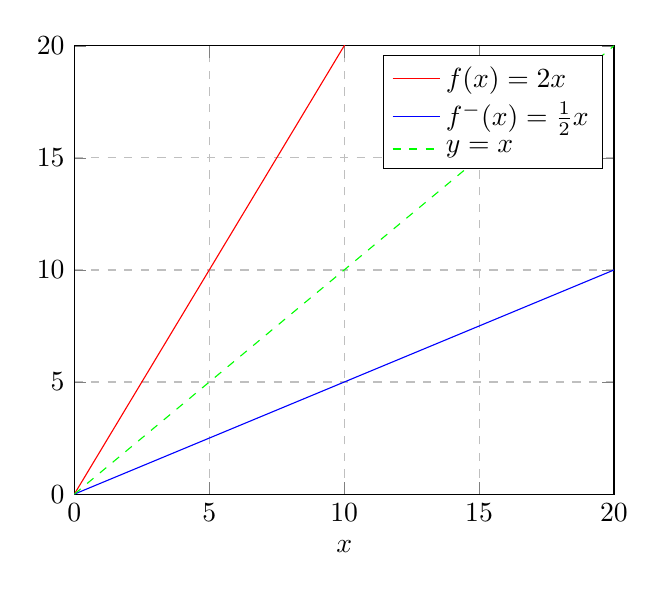
\begin{tikzpicture}
            \begin{axis}[
                legend cell align={left},
                xlabel = \(x\),
                xmin=0, xmax=20,
                ymin=0, ymax=20,
                ymajorgrids=true, xmajorgrids=true,
                grid style=dashed,
            ]
            \addplot[
                domain=0:20,
                color=red,
            ]{2*x};
            \addlegendentry{$f(x)=2x$}
            \addplot[
                domain=0:20,
                color=blue,
            ]{1/2*x};
            \addlegendentry{$f^-(x)=\frac{1}{2}x$}
            \addplot[
                domain=0:20,
                color=green,
                dashed,
            ]{x};
            \addlegendentry{$y=x$}
            \end{axis}
            \end{tikzpicture}
        \end{center}
    
        $f(x)$ and $f^-(x)$ are shown above. $f(x)$ is defined as $f(x)=2x$.
        
        \begin{multicols}{2}
    
        \begin{center}
        \begin{tabular}{|c c|} \hline
           $x$  &  $f(x)$\\\hline
           0  &  0\\
           1  &  2\\
           2  &  4\\
           3  &  6\\
           4  &  8 \\\hline
        \end{tabular}
        \end{center}
    
        \begin{center}
        \begin{tabular}{|c c|} \hline
           $x$  &  $f^-(x)$\\\hline
           0  &  0\\
           2  &  1\\
           4  &  2\\
           6  &  3\\
           8  &  4 \\\hline
        \end{tabular}
        \end{center}
        \end{multicols}
    
        By looking at the graph, the graph of the inverse of a function is a reflection of its original graph along the line $y=x$. In other words, all coordinates' $x$ and $f(x)$ values are switched.
    
        To verify this, we can solve algebraically using the concept that the inverse of the function is formed when all coordinates' independent and the dependent variables on the original function are switched.
        \begin{align}
            f(x)&=2x\\
            x&=2f^-(x)\\
            f^-(x)&=\frac{1}{2}x
        \end{align}
        all dependent and independent variables are switched when the graph is reflected along the line $y=x$, both approaches result in the same inverse function $f^-(x)=\frac{1}{2}x$.

    \subsection{Inverse of Irrational Functions}
        As the previous subsection explained generally, for all functions, by graphing, we can find the inverse by reflecting the original graph along the line $y=x$, or in other words, by re-plot all points as their coordinate values are switched. 

        \begin{center}
            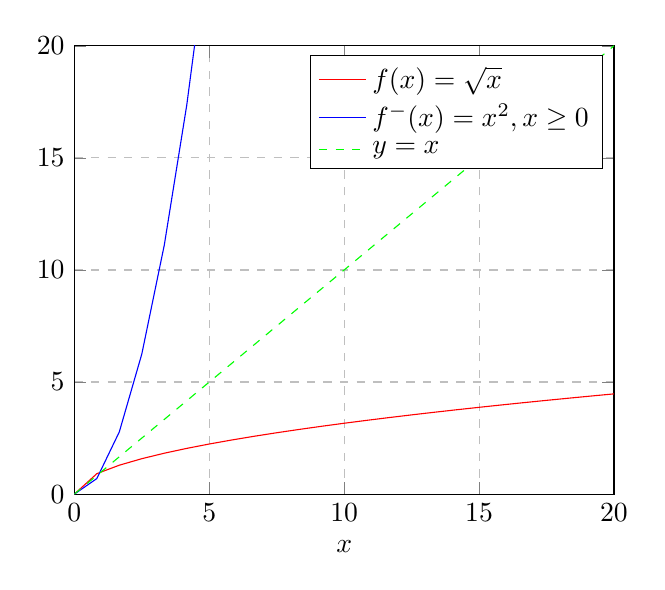
\begin{tikzpicture}
            \begin{axis}[
                legend cell align={left},
                xlabel = \(x\),
                xmin=0, xmax=20,
                ymin=0, ymax=20,
                ymajorgrids=true, xmajorgrids=true,
                grid style=dashed,
            ]
            \addplot[
                domain=0:20,
                color=red,
            ]{sqrt(x)};
            \addlegendentry{$f(x)=\sqrt{x}$}
            \addplot[
                domain=0:20,
                color=blue,
            ]{x^2};
            \addlegendentry{$f^-(x)=x^2, x\geq0$}
            \addplot[
                domain=0:20,
                color=green,
                dashed,
            ]{x};
            \addlegendentry{$y=x$}
            \end{axis}
            \end{tikzpicture}
        \end{center}

        Same pattern appeared. The only 2 points shared by both graphs are $(0,0)$ and $(1,1)$, both lie on the line y=x. which are the invariant points.

        \begin{align}
            f(x)&=\sqrt{x}\\
            x&=\sqrt{f^-(x)}
        \end{align}
        \begin{align*}
             &\because \sqrt{f^-(x)} \in \mathbb{R}\\
             &\therefore f^-(x)\geq0\\
             &\therefore f^-(x)=x^2, x\geq0
        \end{align*}
        Which shows the same graph.
    
    \subsection{Inverse of Polynomial Functions}
        Even though polynomial functions are generally defined as $f(x)=a_nx^n+a_{n-1}x^{n-1}\ldots+a_1x+a_0$. This general form can split into 2 different types of polynomial functions: odd-degree and even-degree polynomials.

        To find the inverse of these 2 types of polynomials, simply reflect the graph along the line $y=x$ is the solution, but both types have different domain or range restrictions. 
        
        \subsubsection{Odd-Degree Polynomials}
            Odd-degree polynomial functions, which $n$ is a positive odd number, have the same domains and ranges:
            \begin{align*}
                &D: \{x\in\mathbb{R}\}\\
                &R: \{f(x)\in\mathbb{R}\}
            \end{align*}
            this indicates that the inverses of odd-degree polynomial functions
            \begin{align*}
                &D: \{x\in\mathbb{R}\}\\
                &R: \{f^-(x)\in\mathbb{R}\}
            \end{align*}
            have the same domains and ranges as their original functions, as shown below:
        \begin{center}
            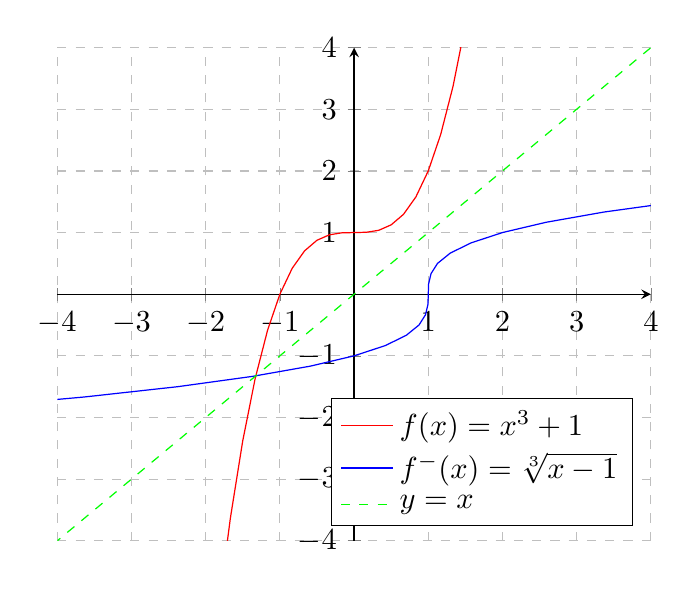
\begin{tikzpicture}[scale=1.1]
            \begin{axis}[
                legend pos = south east,
                legend cell align={left},
                xmin=-4, xmax=4,
                ymin=-4, ymax=4,
                ymajorgrids=true, xmajorgrids=true,
                grid style=dashed,
                axis x line=center,
                axis y line=center,
                xtick={-5,-4,...,5},
                ytick={-5,-4,...,5},
            ]
            \addplot[
                domain=-2:2,
                color=red,
            ]{x^3+1};
            \addlegendentry{$f(x)=x^3+1$};
            \addplot[
                domain=-2:2,
                color=blue,
            ](x^3+1,x);
            \addlegendentry{$f^-(x)=\sqrt[3]{x-1}$}
            \addplot[
                color=green,
                dashed,
            ]{x};
            \addlegendentry{$y=x$};
            \end{axis}
            \end{tikzpicture}
        \end{center}
        
        \subsubsection{Even-Degree Polynomials}
        Even-degree polynomial functions, which $n$ is a positive even number, have only the same domains but not ranges D: $\{x\in\mathbb{R}\}$.
        The ranges of the functions depend on both the $a_n$ values and the maximum or minumum values of the functions. 

        Here is an example of an even-degree polynomial function:
        let $f^-(x)$ be the inverse of $f(x)$ such that $f(x)=2x^4 + 3x^3 - 5x^2 + x - 1$,
        \begin{center}
            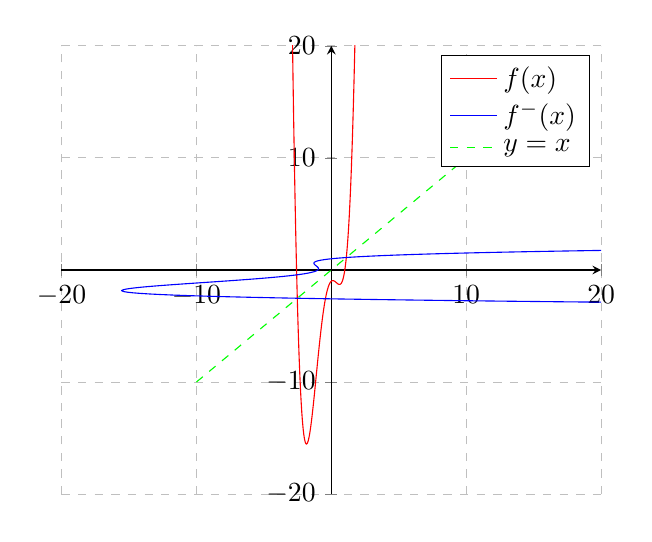
\begin{tikzpicture}[]
            \begin{axis}[
                legend cell align={left},
                xmin=-20, xmax=20,
                ymin=-20, ymax=20,
                ymajorgrids=true, xmajorgrids=true,
                grid style=dashed,
                axis x line=center,
                axis y line=center,
                samples = 200,
            ]
            \addplot[
                color=red,
            ]{2*x^4+3*x^3-5*x^2+x-1};
            \addlegendentry{$f(x)$};
            \addplot[
                color=blue,
            ](2*x^4+3*x^3-5*x^2+x-1,x);
            \addlegendentry{$f^-(x)$};
            \addplot[
                domain=-10:10,
                color=green,
                dashed
            ]{x};
            \addlegendentry{$y=x$};
            \end{axis} 
            \end{tikzpicture}
        \end{center}

        \newpage
        Since the value $a_n$ is greater than 0, and the lowest value of $f(x)$ is approximately -15.532, thus we can say the range of this function is approximately R: $\{f(x)\in\mathbb{R} \:|\: f(x)\geq-15.532\}$.

        In this case, the domain and range of $f(x)$ are
        \begin{align*}
            \centering
            &D: \{x\in\mathbb{R}\}\\
            &R: \{f(x)\in\mathbb{R} \:|\: f(x)\geq-15.532\}
        \end{align*}
        the domain and range of the inverse $f^-(x)$ are
        \begin{align*}
            \centering
            &R: \{x\in\mathbb{R} \:|\: x\geq-15.532\}\\
            &D: \{f^-(x)\in\mathbb{R}\}
        \end{align*}
        we can see that the domains and ranges are switched.

        \newpage
        \subsubsection{Sample Solution of the Inverse of Polynomial Functions}
        To make the life easier, we define $f(x)$ as $f(x)=3x^2+2x+1$, to find the inverse of $f(x)$ which is $f^-(x)$, we switch $x$ to $f(x)$ and change $f(x)$ to $f^-(x)$, then move to where $x$ existed.
        \begin{align}
            f( x) &=3x^{2} +2x+1\\
            x&=3\left( f^{-}( x)\right)^{2} +2\left( f^{-}( x)\right) +1\\
            0&=3\left( f^{-}( x)\right)^{2} +2\left( f^{-}( x)\right) +1-x\\
            f^{-}( x) &=\frac{-2\pm \sqrt{4-4( 3)( 1-x)}}{2( 3)}\\
            f^{-}( x) &=\frac{-2\pm \sqrt{4( 1-3+3x)}}{2( 3)}\\
            f^{-}( x) &=\frac{-2\pm 2\sqrt{3x-2}}{2( 3)}
        \end{align}
        \begin{equation*}
            \therefore f^{-}( x) =\frac{-1\pm \sqrt{3x-2}}{3}
        \end{equation*}
        \begin{center}
            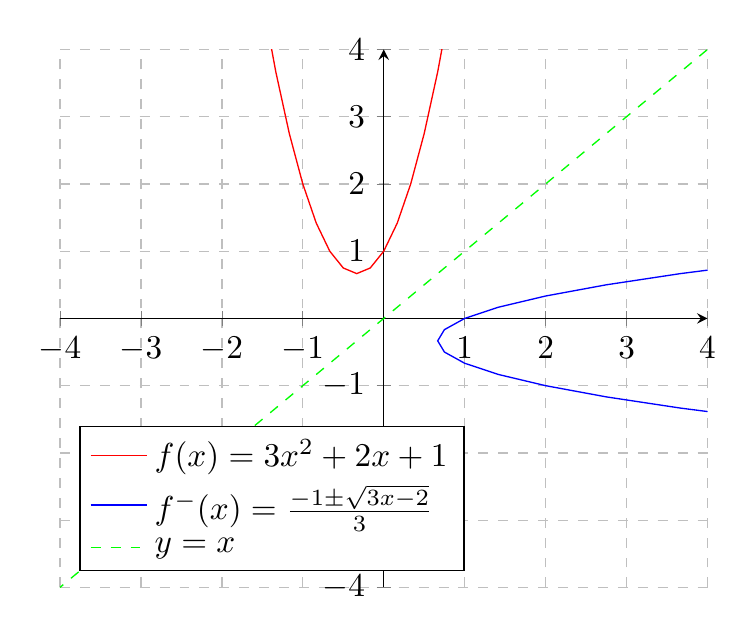
\begin{tikzpicture}[xscale=1.2, yscale=1.2]
            \begin{axis}[
                legend pos = south west,
                legend cell align={left},
                xmin=-4, xmax=4,
                ymin=-4, ymax=4,
                ymajorgrids=true, xmajorgrids=true,
                grid style=dashed,
                axis x line=center,
                axis y line=center,
                xtick={-5,-4,...,5},
                ytick={-5,-4,...,5},
            ]
            \addplot[
                domain=-2:2,
                color=red,
            ]{3*x^2+2*x+1};
            \addlegendentry{$f(x)=3x^2+2x+1$};
            \addplot[
                domain=-2:2,
                color=blue,
            ](3*x^2+2*x+1,x);
            \addlegendentry{$f^{-}( x) =\frac{-1\pm \sqrt{3x-2}}{3}$}
            \addplot[
                color=green,
                dashed,
            ]{x};
            \addlegendentry{$y=x$};
            \end{axis}
            \end{tikzpicture}
        \end{center}
        The graph verifies the equation of the inverse function. 
    
    \subsection{Inverse of Rational Functions}
    Rational functions are functions that are fractions, and both the denominators and the numerators are polynomials. Generally a rational function is defined as
    \begin{equation}
        f(x)=\frac{a_mx^m+a_{m-1}x^{m-1}+\ldots+a_1x+a_0}{b_nx^n+b_{n-1}x^{n-1}+\ldots+b_1x+b_0}
    \end{equation}
    which $m,n\in\mathbb{N}_0$, $b_i$ not all equal to 0. 

    $f(x)=\frac{x^2+x-2}{2x^2-2x-3}$ is an example of rational functions. To find the inverse of $f(x)$, $f^-(x)$, we follow the same steps as the previous section,
    \begin{align}
        f(x)&=\frac{x^2+x-2}{2x^2-2x-3}\\
        x&=\frac{(f^-(x))^2+(f^-(x))-2}{2(f^-(x))^2-2(f^-(x))-3}\\
        2(f^-(x))^2x-2(f^-(x))x-3x&=(f^-(x))^2+(f^-(x))-2
    \end{align}
    \begin{align}
        0&=f^-(x)^2(2x-1)+f^-(x)(-2x-1)-3x+2\\
        f^-(x)&=\frac{-(-2x-1)\pm\sqrt{(-2x-1)^2-4(2x-1)(2-3x)}}{2(2x-1)}\\
        f^-(x)&=\frac{2x+1\pm\sqrt{(4x^2+4x+1)-4(-6x^2+7x-2)}}{2(2x-1)}\\
        f^-(x)&=\frac{2x+1\pm\sqrt{4x^2+4x+1+24x^2-28x+8}}{2(2x-1)}\\
        \therefore f^-(x)&=\frac{2x+1\pm\sqrt{28x^2-24x+9}}{2(2x-1)}
    \end{align}
    
    Same as even-degree polynomial functions, the inverse of rational function can be a relation rather than a function since different $x$ values can have the same $f(x)$ value. 
    
    Because of the denominator $2x^2-2x-3$ of $f(x)$ cannot be 0, then there are 2 vertical asymptotes at
    \begin{align}
        x&=\frac{-(-2)\pm \sqrt{(-2)^2-4(2)(-3)}}{2(2)}\\
        x&=\frac{2\pm \sqrt{4+24}}{2(2)}\\
        x&=\frac{2\pm \sqrt{28}}{2(2)}\\
        x&=\frac{1}{2}\pm\frac{\sqrt{7}}{2}
    \end{align}
    After the $x$ values and $f(x)$ value are switched, the 2 vertical asymptotes of the original equation becomes 2 horizontal asymptotes which are $f^-(x) = \frac{1}{2}\pm\frac{\sqrt{7}}{2}$.
    
    To determine the horizontal asymptotes of $f(x)$, we first divide $m$ by $n$, which in this case is $\frac{1}{1}=1$. When $\frac{m}{n}<1$, there is 1 horizontal asymptote at 0; when $\frac{m}{n}=1$, there is 1 horizontal asymptote at $\frac{a_m}{b_n}$; when $\frac{m}{n}>1$, there is no horizontal asymptote, but a oblique, or a slant asymptote occurs which can be calculated by dividing the numerator by the denominator, and the quotient is the equation of the asymptote. In this scenario, $\frac{m}{n}=1$, which the horizontal asymptote is $f(x)=\frac{a_m}{b_n}=\frac{1}{2}$. Which also indicates that the vertical asymptote of $f^-(x)$ is $x=\frac{1}{2}$.

    \newpage
    Below is the graph of both $f(x)$ and its inverse $f^-(x)$, horizontal and vertical asymptotes are shown as dashed lines as the same colors as the lines,
    \begin{center}
            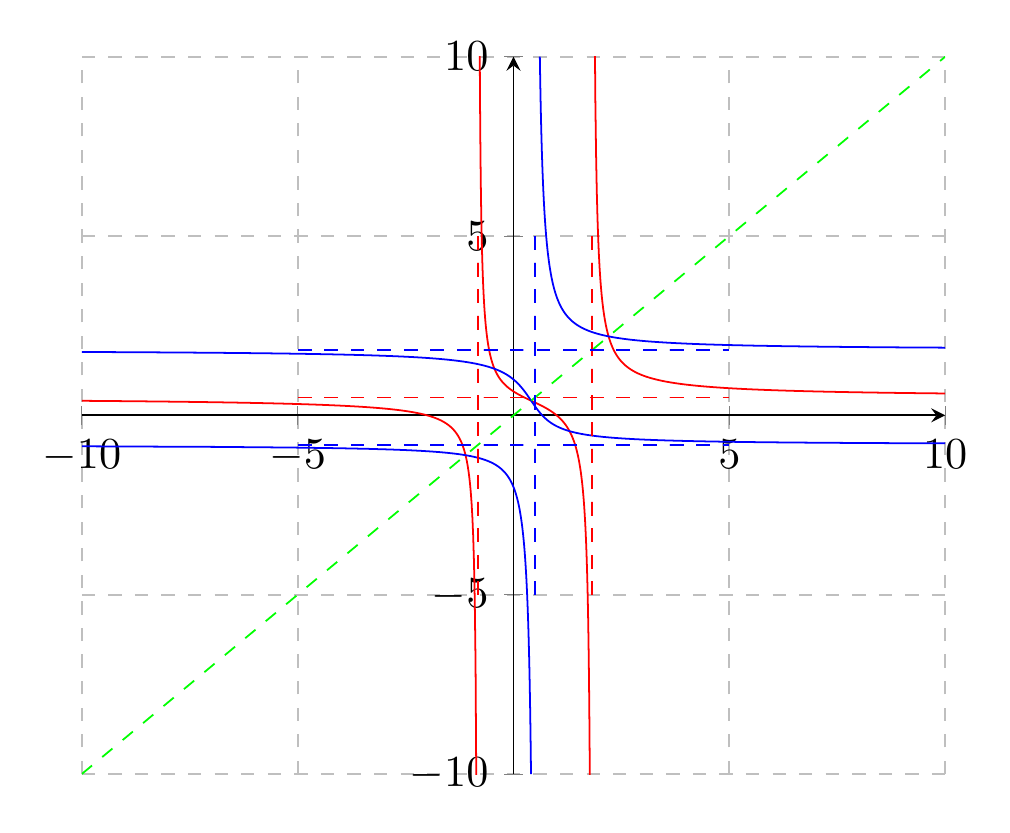
\begin{tikzpicture}[scale = 1.6]
            \begin{axis}[
                legend pos = south east,
                legend cell align={left},
                xmin=-10, xmax=10,
                ymin=-10, ymax=10,
                ymajorgrids=true, xmajorgrids=true,
                grid style=dashed,
                axis x line=center,
                axis y line=center,
                samples = 500,
                %xtick={-20,-4,...,5},
                %ytick={-20,-4,...,5},
                legend style={nodes={scale=0.5, transform shape}}, 
                legend image post style={mark=*}
            ]
            \addplot[
                domain=1.88:10,
                color=red,
            ]{(x^2+x-2)/(2*x^2-2*x-3)};
            \addplot[
                domain=-0.784:1.774,
                color=red,
            ]{(x^2+x-2)/(2*x^2-2*x-3)};
            \addplot[
                domain=-10:-0.861,
                color=red,
            ]{(x^2+x-2)/(2*x^2-2*x-3)};
            \addplot[
                domain=1.88:10,
                color=blue,
            ]((x^2+x-2)/(2*x^2-2*x-3),x);
            \addplot[
                domain=-0.784:1.774,
                color=blue,
            ]((x^2+x-2)/(2*x^2-2*x-3),x);
            \addplot[
                domain=-10:-0.861,
                color=blue,
            ]((x^2+x-2)/(2*x^2-2*x-3),x);
            \addplot[
                domain=-10:10,
                color=green,
                dashed,
            ]{x};
            \addplot[dashed, color=red](0.5+sqrt(7)/2, x);
            \addplot[dashed, color=red](0.5-sqrt(7)/2, x);
            \addplot[dashed, color=blue]{0.5+sqrt(7)/2};
            \addplot[dashed, color=blue]{0.5-sqrt(7)/2};
            
            \addplot[dashed, color=red]{1/2};
            \addplot[dashed, color=blue](1/2, x);
            \end{axis}
            \end{tikzpicture}
    \end{center}
    the red graph represents $f(x)=\frac{x^2+x-2}{2x^2-2x-3}$, the blue graph represents $f^-(x)=\frac{2x+1\pm\sqrt{28x^2-24x+9)}}{2(2x-1)}$, and the green graph represents $y=x$. These graphs proved the answers of the equation of the asymptotes, and reinforced that for all functions, its inverse is always the original graph but reflected along the line $y=x$.

\newpage
\section{Trigonometric Functions and Their Inverses}
    Trigonometric Functions are more complicated than the 3 types of functions mentioned in the previous section, simply exchange $f(x)$ and $x$ values and change $f(x)$ to $f^-(x)$ does not work with trigonometric functions. This section focuses on the graphs, domains and ranges of functions $f(x)=sin(x)$, $g(x)=cos(x)$, $k(x)=tan(x)$,$m(x)=sec(x)$, and their inverses.

    For all types of functions mentioned before, the domains and ranges are simply switched for those functions and their inverses. But for trigonometric functions, to avoid relation of the inverse function instead of a function, we need to either restrict the original trigonometric function, then find the inverse of this domain-restrcted function, or restrict the range of the inverse function after it is reflected along the $y=x$ line or all y-x values are switched. 

    \\
    Here are the trigonometric functions:
    \begin{center}
        \begin{tabular}{c|c|c|c}
           Original Functions & Reciprocal  & Inverse  & Inverse Reciprocal  \\
           $sin(x)$  & $csc(x)$ & $arcsin(x)$ & $arccsc(x)$\\
            $cos(x)$ & $sec(x)$ & $arccos(x)$ & $arcsec(x)$\\
            $tan(x)$ & $cot(x)$ & $arctan(x)$ & $arccot(x)$
    \end{tabular}
    \end{center}
    
    \\ 
    Derivatives of the functions above:
    \begin{center}
        \begin{tabular}{c|c|c|c}
           Original Functions & Reciprocal  & Inverse  & Inverse Reciprocal  \\
           $cos(x)$  & $-cot(x)csc(x)$ & $\frac{1}{\sqrt{1-x^2}}$ & $-\frac{1}{|x|\sqrt{x^2-1}}$\\
            $-sin(x)$ & $tan(x)sec(x)$ & $-\frac{1}{\sqrt{1-x^2}}$ & $\frac{1}{|x|\sqrt{x^2-1}}$\\
            $sec^2(x)$ & $-csc^2(x))$ & $\frac{1}{1+x^2}$ & $-\frac{1}{1+x^2}$
    \end{tabular}
    \end{center}

    \\
    Related derivatives will be proved.

    \newpage
    \subsection{Sine and Its Inverse Arcsine}
    \label{sec:arcsine}
        \begin{center}
                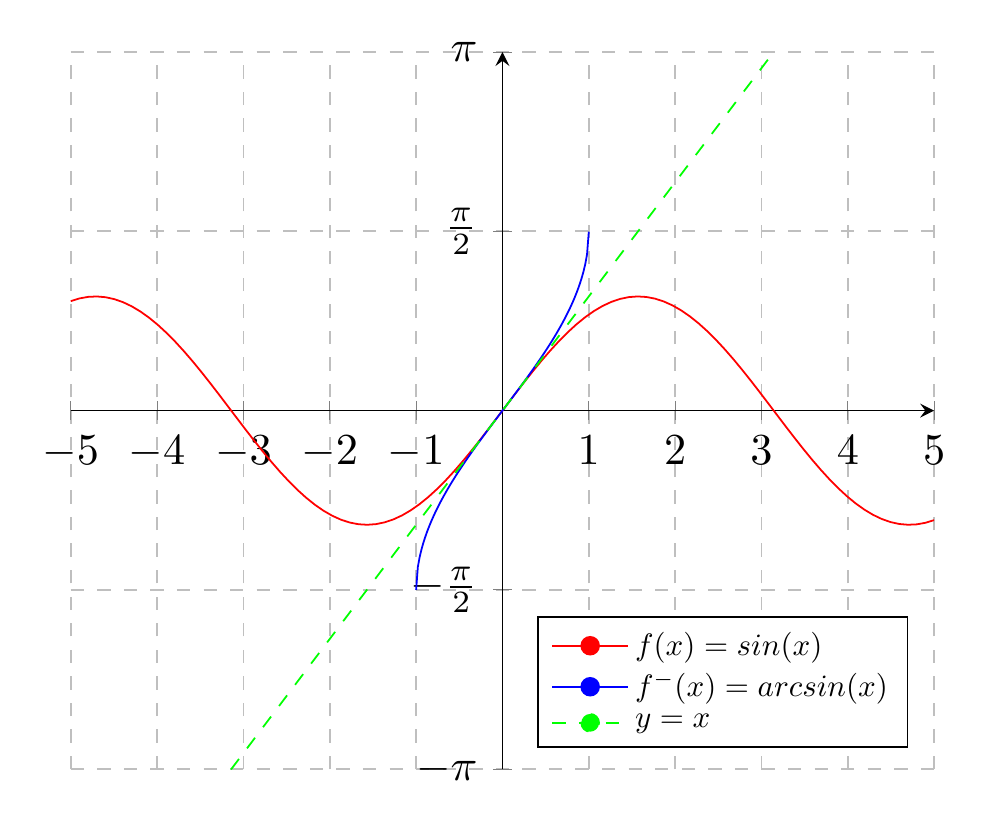
\begin{tikzpicture}[scale = 1.6]
                \begin{axis}[
                    legend pos = south east,
                    legend cell align={left},
                    xmin=-5, xmax=5,
                    ymin=-pi, ymax=pi,
                    ymajorgrids=true, xmajorgrids=true,
                    grid style=dashed,
                    axis x line=center,
                    axis y line=center,
                    samples = 100,
                    xtick={-5,-4,...,5},
                    ytick={-pi, -(1/2)*pi, (1/2)*pi, pi},
                    yticklabels={$-\pi$,$-\frac{\pi}{2}$,$\frac{\pi}{2}$,$\pi$},
                    legend style={nodes={scale=0.7, transform shape}}, 
                    legend image post style={mark=*}
                ]
                \addplot[
                    domain=-5:5,
                    color=red,
                ]{sin(deg(x))};
                \addlegendentry{$f(x)=sin(x)$};
                \addplot[
                    domain=-1:1,
                    color=blue,
                ]{asin(x)/180*pi};
                \addlegendentry{$f^-(x)=arcsin(x)$}
                \addplot[
                    domain=-5:5,
                    color=green,
                    dashed,
                ]{x};
                \addlegendentry{$y=x$};
                \end{axis}
                \end{tikzpicture}
        \end{center}
        As shown, if we simply reflect $f(x)$ along the line $y=x$, then $f^-(x)$ turns into a relation not a function, the range of $arcsine(x)$ is restricted to $[-\frac{\pi}{2}, \frac{\pi}{2}]$ in order to make it a function.

        Thus, the domain and range of $sin(x)$ are
        \begin{align*}
                &D: \{x\in\mathbb{R}\}\\
                &R: \{sin(x)\in\mathbb{R}\:|\:sin(x)\in [-1,1]\}
        \end{align*}
        the domain and range of $arcsin(x)$ are
        \begin{align*}
                &D: \{x\in\mathbb{R}\:|\:x\in [-1,1]\}\\
                &R: \{arcsin(x)\in\mathbb{R}\:|\:arcsin(x)\in [-\frac{\pi}{2}, \frac{\pi}{2}]\}
        \end{align*}
        The domain of $arcsin(x)$ is the range of $sin(x)$, and the range of $arcsin(x)$ is half of the period of $sin(x)$.

        
    \subsection{Cosine and Its Inverse Arccosine}
    \label{sec:arccosine}
    \begin{center}
                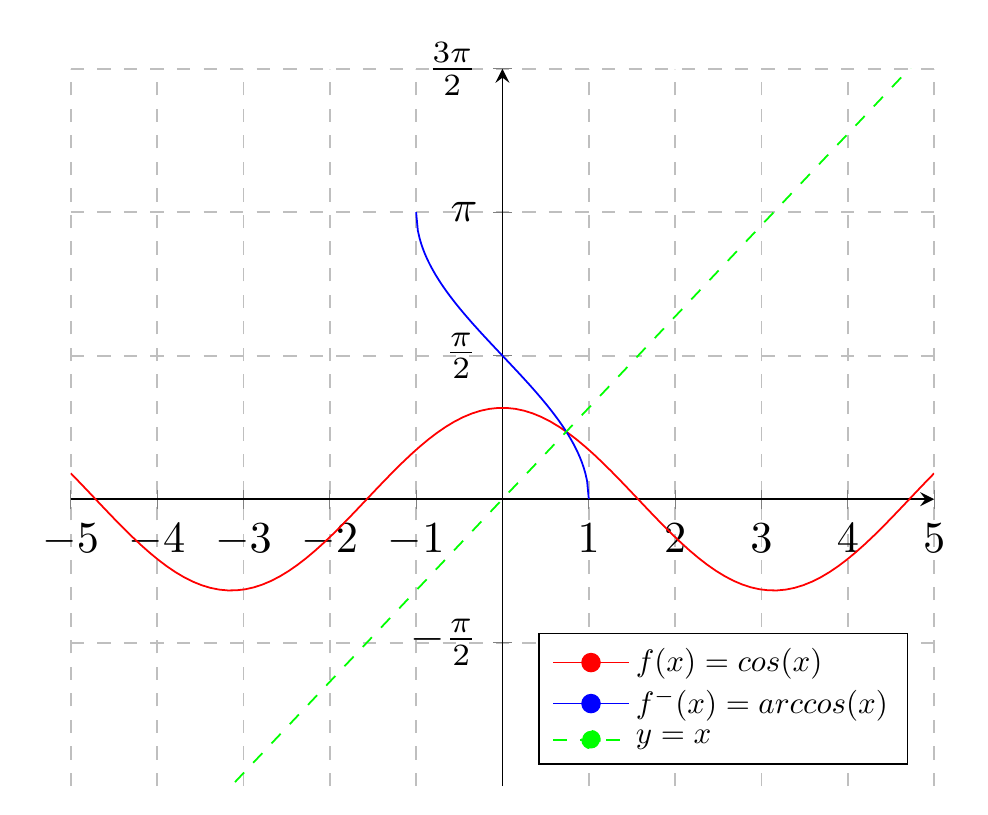
\begin{tikzpicture}[scale = 1.6]
                \begin{axis}[
                    legend pos = south east,
                    legend cell align={left},
                    xmin=-5, xmax=5,
                    ymin=-pi, ymax=1.5*pi,
                    ymajorgrids=true, xmajorgrids=true,
                    grid style=dashed,
                    axis x line=center,
                    axis y line=center,
                    samples = 100,
                    xtick={-5,-4,...,5},
                    ytick={-(1/2)*pi, (1/2)*pi, pi, (3/2)*pi},
                    yticklabels={$-\frac{\pi}{2}$,$\frac{\pi}{2}$,$\pi$,$\frac{3\pi}{2}$},
                    legend style={nodes={scale=0.7, transform shape}}, 
                    legend image post style={mark=*}
                ]
                \addplot[
                    domain=-5:5,
                    color=red,
                ]{cos(deg(x))};
                \addlegendentry{$f(x)=cos(x)$};
                \addplot[
                    domain=-1:1,
                    color=blue,
                ]{acos(x)/180*pi};
                \addlegendentry{$f^-(x)=arccos(x)$}
                \addplot[
                    domain=-5:5,
                    color=green,
                    dashed,
                ]{x};
                \addlegendentry{$y=x$};
                \end{axis}
                \end{tikzpicture}
        \end{center}
        Same as $sin(x$) and $arcsin(x)$, the range of $arccos(x)$ is restricted to $[0,\pi]$ to make it a function not a relation. 

        Thus, the domain and range of $cos(x)$ are
        \begin{align*}
                &D: \{x\in\mathbb{R}\}\\
                &R: \{cos(x)\in\mathbb{R}\:|\:cos(x)\in [-1,1]\}
        \end{align*}
        the domain and range of $arccos(x)$ are
        \begin{align*}
                &D: \{x\in\mathbb{R}\:|\:x\in [-1,1]\}\\
                &R: \{arccos(x)\in\mathbb{R}\:|\:arccos(x)\in [0, \pi]\}
        \end{align*}

        The domain of $arccos(x)$ is the range of $cos(x)$, and the range of $arccos(x)$ is half of the period of $cos(x)$.
    
    \subsection{Tangent and Its Inverse Arctangent}
    
    \begin{center}
                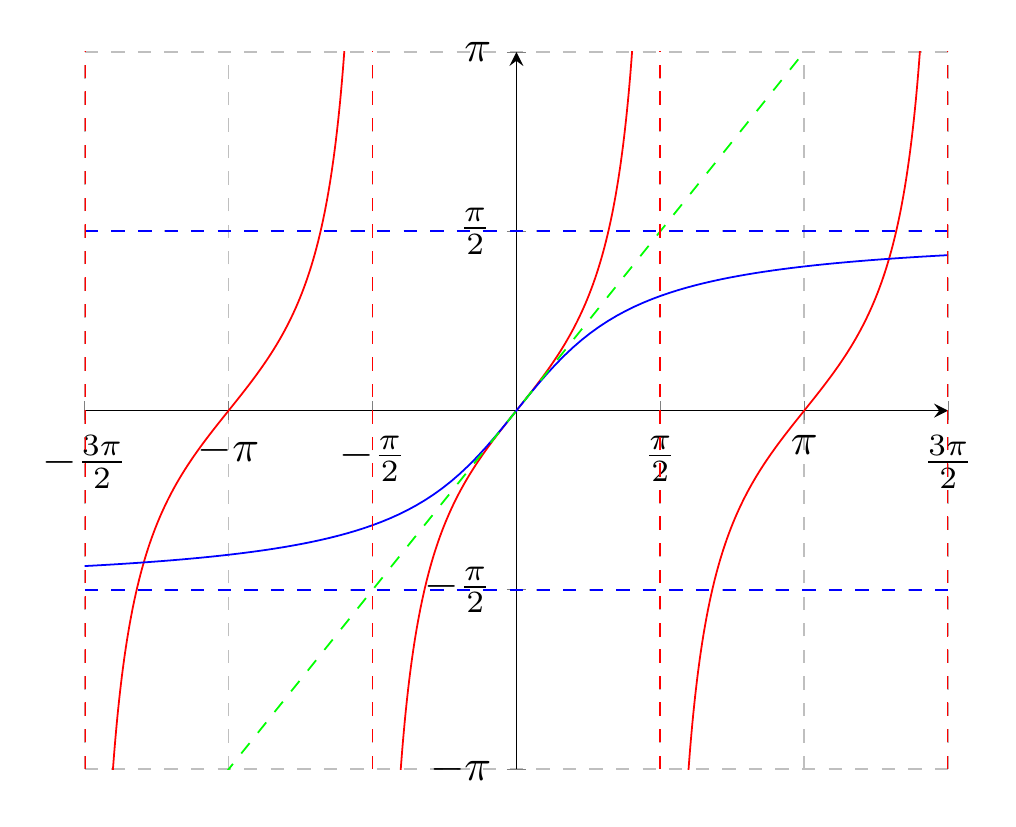
\begin{tikzpicture}[scale = 1.6]
                \begin{axis}[
                    legend pos = south east,
                    legend cell align={left},
                    xmin=-1.5*pi, xmax=1.5*pi,
                    ymin=-pi, ymax=pi,
                    ymajorgrids=true, xmajorgrids=true,
                    grid style=dashed,
                    axis x line=center,
                    axis y line=center,
                    samples = 100,
                    xtick={-(3/2)*pi, -pi, -(1/2)*pi,(1/2)*pi, pi, (3/2)*pi},
                    ytick={-pi, -(1/2)*pi, (1/2)*pi, pi},
                    xticklabels={$-\frac{3\pi}{2}$,$-\pi$,$-\frac{\pi}{2}$,$\frac{\pi}{2}$,$\pi$,$\frac{3\pi}{2}$},
                    yticklabels={$-\pi$,$-\frac{\pi}{2}$,$\frac{\pi}{2}$,$\pi$},
                    legend style={nodes={scale=0.7, transform shape}}, 
                    legend image post style={mark=*}
                ]
                \foreach \i in {0,...,4} \addplot[color=red, domain={((\i-2)*pi-rad(atan(4))*ceil(\i/4))}:{((\i-2)*pi+rad(atan(4))*ceil((4-\i)/4))},smooth]{tan(\x r)};
                \addplot[
                    domain=-1.5*pi:1.5*pi,
                    color=blue,
                ]{atan(x)/180*pi};
                \addplot[
                    domain=-5:5,
                    color=green,
                    dashed,
                ]{x};
                \foreach \i in {-pi/2, pi/2} \addplot[dashed, color=blue]{\i};
                \foreach \i in {-3*pi/2, -pi/2, pi/2, 3*pi/2} \addplot[dashed, color=red](\i, x);
                \end{axis}
                \end{tikzpicture}
        \end{center}
        Red graph represents $tan(x)$, blue graph represents $arctan(x)$, and green dashed line represents $y=x$. The range of $arctan(x)$ is limited to the interval $(-\frac{\pi}{2},\frac{\pi}{2})$ to avoid relation. 

        Then, the Domain and Range of $\displaystyle tan( x)$ are:
            \begin{align*}
                D&:\ \left\{x\in \mathbb{R}\:|\:x\neq \left(\frac{\pi }{2} +k\pi \right) ,k\in \mathbb{Z}\right\}\\
                R&:\ \{tan(x)\in \mathbb{R} \}
            \end{align*}
        the Domain and Range of $\displaystyle arctan( x)$ are:
            \begin{align*}
                D&:\ \{x\in \mathbb{R}\}\\
                R&:\ \left\{arctan(x)\in \mathbb{R}\:|\:\arctan(x)\in \left( -\frac{\pi }{2} ,\frac{\pi }{2}\right)\right\}
            \end{align*}

        The domain of $arctan(x)$ is the range of $tan(x)$.
    
    
    \subsection{Secant and Its Inverse Arcsecant}

    \begin{center}
                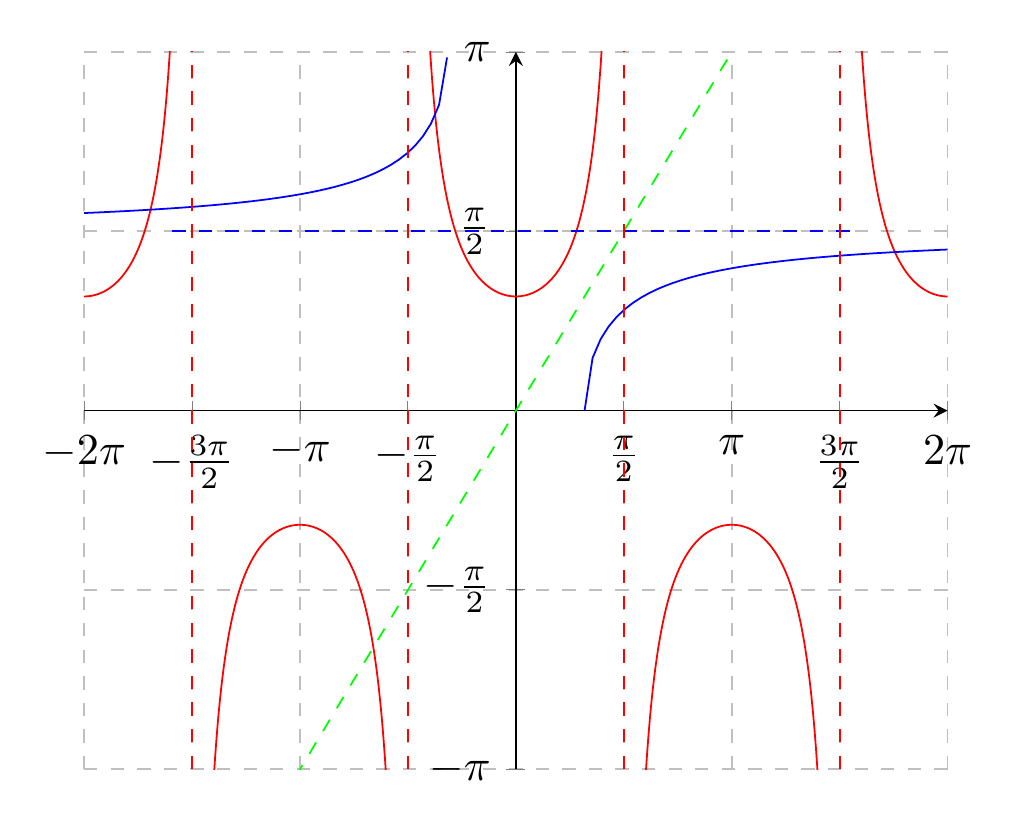
\begin{tikzpicture}[scale = 1.6]
                \begin{axis}[
                    legend pos = south east,
                    legend cell align={left},
                    xmin=-2*pi, xmax=2*pi,
                    ymin=-pi, ymax=pi,
                    ymajorgrids=true, xmajorgrids=true,
                    grid style=dashed,
                    axis x line=center,
                    axis y line=center,
                    samples = 100,
                    xtick={-2*pi,-(3/2)*pi,-pi, -(1/2)*pi, (1/2)*pi, pi, (3/2)*pi, 2*pi},
                    ytick={-pi, -(1/2)*pi, (1/2)*pi, pi},
                    xticklabels={$-2\pi$,$-\frac{3\pi}{2}$,$-\pi$,$-\frac{\pi}{2}$,$\frac{\pi}{2}$,$\pi$,$\frac{3\pi}{2}$,$2\pi$},
                    yticklabels={$-\pi$,$-\frac{\pi}{2}$,$\frac{\pi}{2}$,$\pi$,$\frac{3\pi}{2}$},
                    legend style={nodes={scale=0.7, transform shape}}, 
                    legend image post style={mark=*},
                ]
                %\foreach \i in {-1,0,1,2,3,4,5} \addplot [color=red,domain={(pi*(\i-2)-acos(1/4)*ceil(\i/4))}:{(pi*(\i-2)+acos(1/4)*ceil((4-\i)/4))/pi*2},smooth] {cos(1/x)/180*pi};
                \foreach \i in {0,...,4} \addplot[color=red, domain={((\i-2)*pi-rad(acos(1/4))*ceil(\i/4))}:{((\i-2)*pi+rad(acos(1/4))*ceil((4-\i)/4))},smooth] {sec(\x r)};
                \addplot[
                    domain=-4*pi:-1,
                    color=blue,
                ]{acos(1/x)/180*pi};
                \addplot[
                    domain=1:4*pi,
                    color=blue,
                ]{acos(1/x)/180*pi};
                \addplot[
                    domain=-5:5,
                    color=green,
                    dashed,
                ]{x};
                
                \foreach \i in {pi/2} \addplot[dashed, color=blue]{\i};
                \foreach \i in {-3*pi/2, -pi/2, pi/2, 3*pi/2} \addplot[dashed, color=red](\i, x);
                \end{axis}
                \end{tikzpicture}
        \end{center}
        Red graph represents $sec(x)$, blue graph represents $arcsec(x)$, and green dashed line represents $y=x$. The range of $arcsec(x)$ is limited to the interval $[0,\pi]$ to avoid relation, but the range of $arcsec(x)$ does not belong to the entire interval. 

        Then, the Domain and Range of $\displaystyle sec( x)$ are:
            \begin{align*}
                D&:\ \left\{x\in \mathbb{R}\:|\:x\neq \left(\frac{\pi }{2} +k\pi \right) ,k\in \mathbb{Z}\right\}\\
                R&: \{sec(x)\in \mathbb{R}\:|\:sec(x)\in ( -\infty ,-1] \cup [ 1,\infty )\}
            \end{align*}
        the Domain and Range of $\displaystyle arcsec( x)$ are:
            \begin{align*}
                D&: \{x\in \mathbb{R}\:|\:x\in ( -\infty ,-1] \cup [ 1,\infty )\}\\
                R&: \{arcsec(x)\in \mathbb{R}\:|\:arcsec(x)\in [0,\frac{\pi}{2})\cup(\frac{\pi}{2},\pi]\}
            \end{align*}
            
        The domain of $arcsec(x)$ is the range of $sec(x)$.

\newpage
\section{Derivative of Inverse Sine Function}
    In this section, we will be deriving the formula for $\frac{d}{dx}(sin^-(x))$ using the inverse functions theorem, the unit circle, and the Pythagorean identity.

    $\displaystyle \frac{d}{dx}\left( sin^{-}( x)\right)$ is equivalent to $\displaystyle \frac{dy}{dx}$ of the equation $\displaystyle \ y\ =sin^{-}( x)$, x is the independent variable and y is t he dependent variable,
     \begin{align}
        \label{yisarcsin}
        \ y\ &=sin^{-}( x)\\
        sin( y) &=sin\left( sin^{-}( x)\right)
    \end{align}
    using the inverse functions theorem $\displaystyle f\left( f^{-}( x)\right) =x$,
    \begin{align}
        \label{eq:siny}
        sin(y)=x
    \end{align}
    differentiate both sides using the identity $\displaystyle sin'( x) =cos( x) \times ( x) '$.%, and the chain rule $(x^n)^{'} = n x^{n-1} (x)^{'}$,
     \begin{align}
        ( sin( y))^{'} &=( x)^{'}\\
        cos( y) \times \frac{dy}{dx} &=1\\
        \frac{dy}{dx} &=\frac{1}{cos( y)}
    \end{align}
    we must change $cos(y)$ in terms of $x$ instead of $y$ since $y$ is the dependent variable and $x$ is the independent variable.

    \subsection{the Pythagorean Theorem}
    \label{sec:pytha}
    The Pythagorean Theorem states that for all right angle triangles, the sum of the square of 2 right angle sides is equal to the square of the hypotenuse,
    \begin{center}
        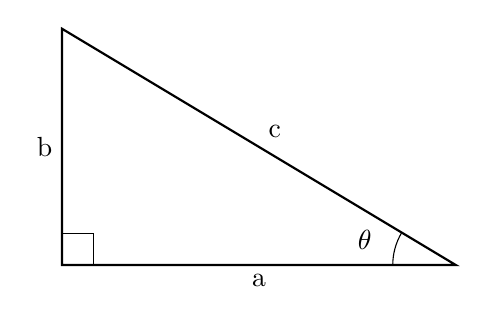
\begin{tikzpicture}
            \coordinate (A) at (0,3);
            \coordinate (B) at (5,0);
            \coordinate (C) at (0,0);
            \draw[thick] (A) -- (B) -- (C) -- cycle;
            
            \tkzLabelSegment[above right](A,B){c}
            \tkzLabelSegment[left](A,C){b}
            \tkzLabelSegment[below](B,C){a}

            \tkzMarkRightAngle[size=.4](A,C,B)
            \tkzMarkAngle[mark=none, size=0.8cm](A,B,C)
            \tkzLabelAngle[pos=1.2](A,B,C){$\theta$}
        \end{tikzpicture}
    \end{center}
    in this case, $a^2+b^2=c^2$. Let $\theta$ be any angle in the interval $(0,\frac{\pi}{2})$, then $sin(\theta)=\frac{b}{c}$, $cos(\theta)=\frac{a}{c}$, and $tan(\theta)=\frac{b}{a}$.

    \subsection{the Unit Circle and the Pythagorean Identity}
    \label{sec:4.2}
    Now we can apply the concept of the Pythagorean Theorem into the unit circle.

    Unit circle, a circle that has a radius of 1,
    \begin{center}
        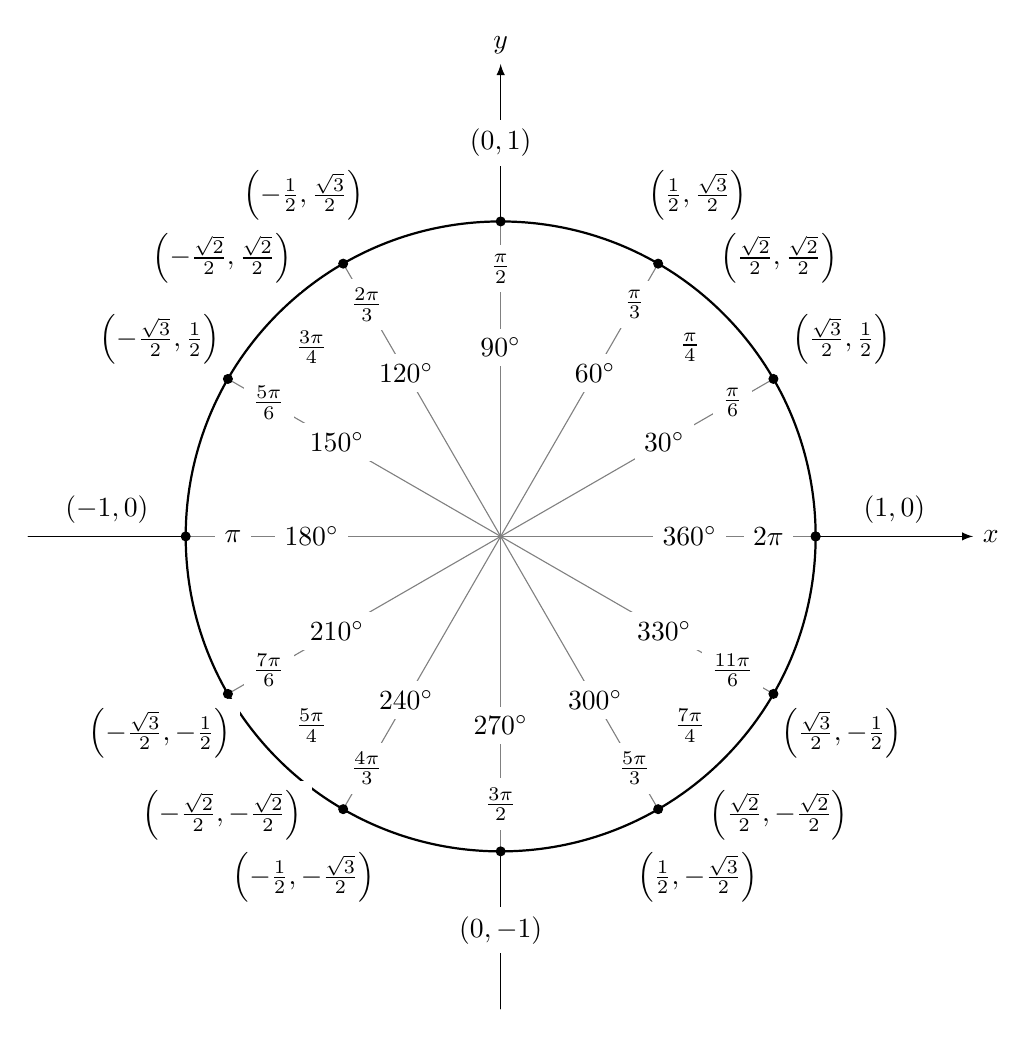
\begin{tikzpicture}[scale=4,cap=round,>=latex]
        % draw the coordinates
        \draw[->] (-1.5cm,0cm) -- (1.5cm,0cm) node[right,fill=white] {$x$};
        \draw[->] (0cm,-1.5cm) -- (0cm,1.5cm) node[above,fill=white] {$y$};

        % draw the unit circle
        \draw[thick] (0cm,0cm) circle(1cm);

        \foreach \x in {0,30,...,360} {
                % lines from center to point
                \draw[gray] (0cm,0cm) -- (\x:1cm);
                % dots at each point
                \filldraw[black] (\x:1cm) circle(0.4pt);
                % draw each angle in degrees
                \draw (\x:0.6cm) node[fill=white] {$\x^\circ$};
        }

        % draw each angle in radians
        \foreach \x/\xtext in {
            30/\frac{\pi}{6},
            45/\frac{\pi}{4},
            60/\frac{\pi}{3},
            90/\frac{\pi}{2},
            120/\frac{2\pi}{3},
            135/\frac{3\pi}{4},
            150/\frac{5\pi}{6},
            180/\pi,
            210/\frac{7\pi}{6},
            225/\frac{5\pi}{4},
            240/\frac{4\pi}{3},
            270/\frac{3\pi}{2},
            300/\frac{5\pi}{3},
            315/\frac{7\pi}{4},
            330/\frac{11\pi}{6},
            360/2\pi}
                \draw (\x:0.85cm) node[fill=white] {$\xtext$};

        \foreach \x/\xtext/\y in {
            % the coordinates for the first quadrant
            30/\frac{\sqrt{3}}{2}/\frac{1}{2},
            45/\frac{\sqrt{2}}{2}/\frac{\sqrt{2}}{2},
            60/\frac{1}{2}/\frac{\sqrt{3}}{2},
            % the coordinates for the second quadrant
            150/-\frac{\sqrt{3}}{2}/\frac{1}{2},
            135/-\frac{\sqrt{2}}{2}/\frac{\sqrt{2}}{2},
            120/-\frac{1}{2}/\frac{\sqrt{3}}{2},
            % the coordinates for the third quadrant
            210/-\frac{\sqrt{3}}{2}/-\frac{1}{2},
            225/-\frac{\sqrt{2}}{2}/-\frac{\sqrt{2}}{2},
            240/-\frac{1}{2}/-\frac{\sqrt{3}}{2},
            % the coordinates for the fourth quadrant
            330/\frac{\sqrt{3}}{2}/-\frac{1}{2},
            315/\frac{\sqrt{2}}{2}/-\frac{\sqrt{2}}{2},
            300/\frac{1}{2}/-\frac{\sqrt{3}}{2}}
                \draw (\x:1.25cm) node[fill=white] {$\left(\xtext,\y\right)$};

        % draw the horizontal and vertical coordinates
        % the placement is better this way
        \draw (-1.25cm,0cm) node[above=1pt] {$(-1,0)$}
              (1.25cm,0cm)  node[above=1pt] {$(1,0)$}
              (0cm,-1.25cm) node[fill=white] {$(0,-1)$}
              (0cm,1.25cm)  node[fill=white] {$(0,1)$};
    \end{tikzpicture}
    \end{center}

    \newpage
    Choose any related acute angle in the unit circle, let $\theta$ be the angle,
    \begin{center}
        \begin{tikzpicture}[scale=2.5]
            \draw[step=.5cm,gray,very thin,dashed] (-1.4,-1.4) grid (1.4,1.4);
            \draw (0,0) -- (3mm,0mm)
            arc [start angle=0, end angle=30, radius=3mm] -- cycle;
            \node at (23:3.7mm) {$\theta$};
            \draw[->] (-1.5,0) -- (1.5,0) coordinate (x axis)node[right]{$x$};
            \draw[->] (0,-1.5) -- (0,1.5) coordinate (y axis)node[above]{$y$};
            \draw (0,0) circle [radius=1cm];
            \draw[very thick,red]
            (30:1cm) -- node[right=1pt,fill=white] {$b$} (30:1cm |- x axis);
            \draw[very thick,blue]
            (30:1cm |- x axis) -- node[below=2pt,fill=white] {$a$} (0,0);
            \path [name path=upward line] (1,0) -- (1,1);
            \path [name path=sloped line] (0,0) -- (30:1cm);
            \draw [very thick,black] (0,0) -- (0.866, 0.5);
            \coordinate (O) at (0,0);
            \coordinate (P) at (0.866,0.5);
            \tkzLabelSegment[above left](O,P){r}
            \foreach \x/\xtext in {-1, -0.5/-\frac{1}{2}, 1}
            \draw (\x cm,1pt) -- (\x cm,-1pt) node[anchor=north,fill=white] {$\xtext$};
            \foreach \y/\ytext in {-1, -0.5/-\frac{1}{2}, 0.5/\frac{1}{2}, 1}
            \draw (1pt,\y cm) -- (-1pt,\y cm) node[anchor=east,fill=white] {$\ytext$};
        \end{tikzpicture}
    \end{center}
    since $r=1$, thus $sin(\theta)=\frac{b}{r}=b$, $cos(\theta)=\frac{a}{r}=a$. Which means we can rewrite the adjacent side length of the triangle formed inside the unit circle with respect to $\theta$ as $cos(\theta)$, and the opposite side length as $sin(\theta)$,
    \begin{center}
        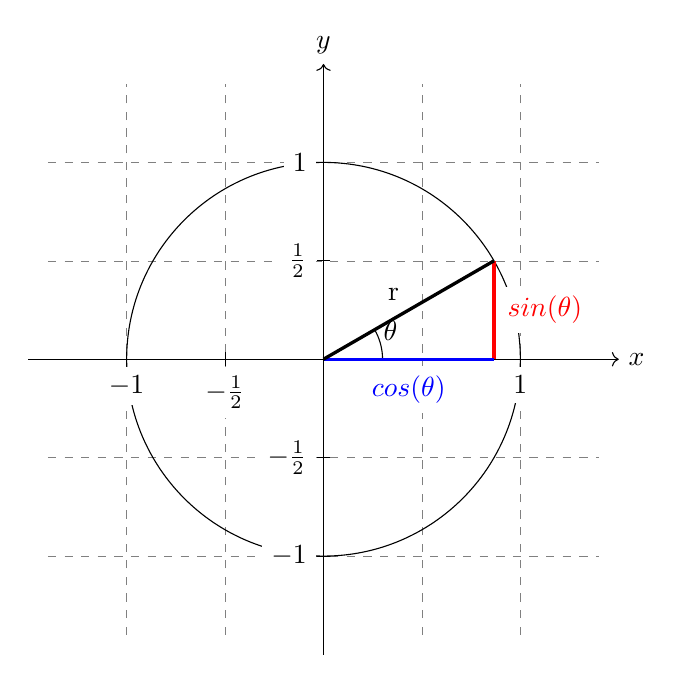
\begin{tikzpicture}[scale=2.5]
            \draw[step=.5cm,gray,very thin,dashed] (-1.4,-1.4) grid (1.4,1.4);
            \draw (0,0) -- (3mm,0mm)
            arc [start angle=0, end angle=30, radius=3mm] -- cycle;
            \node at (23:3.7mm) {$\theta$};
            \draw[->] (-1.5,0) -- (1.5,0) coordinate (x axis)node[right]{$x$};
            \draw[->] (0,-1.5) -- (0,1.5) coordinate (y axis)node[above]{$y$};
            \draw (0,0) circle [radius=1cm];
            \draw[very thick,red]
            (30:1cm) -- node[right=1pt,fill=white] {$sin(\theta)$} (30:1cm |- x axis);
            \draw[very thick,blue]
            (30:1cm |- x axis) -- node[below=2pt,fill=white] {$cos(\theta)$} (0,0);
            \path [name path=upward line] (1,0) -- (1,1);
            \path [name path=sloped line] (0,0) -- (30:1cm);
            \draw [very thick,black] (0,0) -- (0.866, 0.5);
            \coordinate (O) at (0,0);
            \coordinate (P) at (0.866,0.5);
            \tkzLabelSegment[above left](O,P){r}
            \foreach \x/\xtext in {-1, -0.5/-\frac{1}{2}, 1}
            \draw (\x cm,1pt) -- (\x cm,-1pt) node[anchor=north,fill=white] {$\xtext$};
            \foreach \y/\ytext in {-1, -0.5/-\frac{1}{2}, 0.5/\frac{1}{2}, 1}
            \draw (1pt,\y cm) -- (-1pt,\y cm) node[anchor=east,fill=white] {$\ytext$};
        \end{tikzpicture}
    \end{center}

    Now applying the Pythagorean Theorem,
    \begin{center}
        \begin{align}
            a^2+b^2&=r^2\\
            cos^2(\theta)+sin^2(\theta)&=1
        \end{align}
    \end{center}
    the Pythagorean Identity is proved which is $cos^2(\theta)+sin^2(\theta)=1$.

    \subsection{Change $\frac{dy}{dx}$ to in Terms of $x$}
    Since $\frac{dy}{dx} =\frac{1}{cos( y)}$, we need to change $cos(y)$ to in terms of x.

    Using the Pythagorean Identity derived previously,
    \begin{center}
        \begin{align}
            cos^2(\theta)+sin^2(\theta)&=1\\
            cos^2(\theta)&=1-sin^2(\theta)\\
            cos(\theta)&=\pm\sqrt{1-sin^2(\theta)}
        \end{align}
    \end{center}
    thus, the general form of $cos(\theta)$ is $\pm\sqrt{1-sin^2(\theta)}$.

    When changing $\theta$ to $y$, there are some restrictions. As shown in Section \ref{sec:arcsine}, the range of $arcsin(x)$, or $sin^-(x)$ is $R: \{arcsin(x)\in\mathbb{R}\:|\:arcsin(x)\in [-\frac{\pi}{2}, \frac{\pi}{2}]\}$. At 
    \eqref{yisarcsin} we found that $y$ is the arcsine of x, which means the range of $y$ is $R: \{y\in\mathbb{R}\:|\:y\in [-\frac{\pi}{2}, \frac{\pi}{2}]\}$.
    
    By looking at the unit circle,
    \begin{center}
        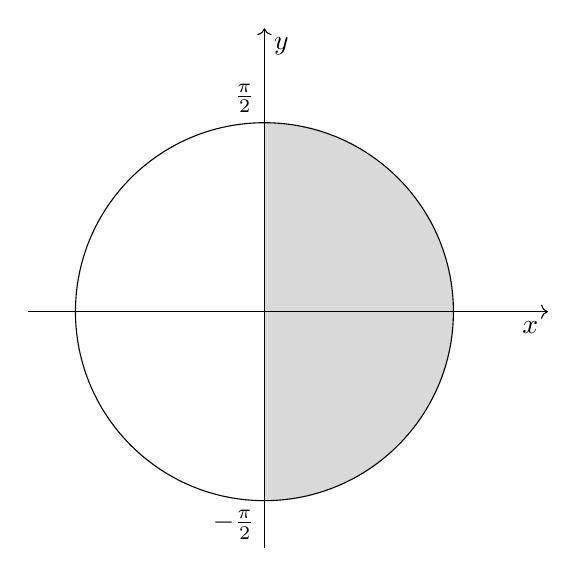
\begin{tikzpicture}[scale=2.4]
            \fill[gray!30] (0,0) -- (1,0) arc (0:90:1);
            \fill[gray!30] (0,0) -- (0,-1) arc (270:360:1);
            \draw[->] (-1.25,0) -- (1.5,0) node[below left] {$x$};
            \draw[->] (0,-1.25) -- (0,1.5) node[below right] {$y$};
            \draw (0,0) circle [radius=1]; 
            \coordinate[label=above left:$\frac{\pi}{2}$] (Q) at (0,1);
            \coordinate[label=below left:$-\frac{\pi}{2}$] (P) at (0,-1);
        \end{tikzpicture}
    \end{center}
    as proved in Section \ref{sec:4.2}, for any point $P$ on the unit circle, the coordinate of $P$ is $cos(x), sin(x)$, thus within $y$'s range, the $x$ value must $\geq0$, or in other words, $cos(x)$ always $\geq0$.
    
    Also, as derived at \eqref{eq:siny}, we can substitute $x$ to $sin(y)$.

    Therefore, we can convert $cos(y)$ to $\sqrt{1-x^2}$.

    Substituting $\sqrt{1-x^2}$ into $cos(y)$, we get:
    \begin{center}
        \begin{equation}
            \frac{dy}{dx} =\frac{1}{\sqrt{1-x^2}}
        \end{equation}
    \end{center}
    converting back, 
    \begin{center}
        \begin{equation}
            \label{eq:dasin}
            \frac{d}{dx}(sin^-(x)) =\frac{1}{\sqrt{1-x^2}}
        \end{equation}
    \end{center}

    \subsection{Another Approach}
    Using the concepts of the Pythagorean Theorem, and the Unit Circle, we can find $\frac{d}{dx}(sin^-(x))$ in another way.

    Since $sin(y)=x$ derived at \eqref{eq:siny}, and the radius of the unit circle is always 1, then,
    \begin{center}
        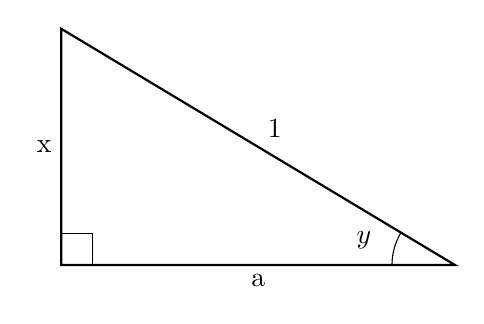
\begin{tikzpicture}
            \coordinate (A) at (0,3);
            \coordinate (B) at (5,0);
            \coordinate (C) at (0,0);
            \draw[thick] (A) -- (B) -- (C) -- cycle;
            
            \tkzLabelSegment[above right](A,B){1}
            \tkzLabelSegment[left](A,C){x}
            \tkzLabelSegment[below](B,C){a}

            \tkzMarkRightAngle[size=.4](A,C,B)
            \tkzMarkAngle[mark=none, size=0.8cm](A,B,C)
            \tkzLabelAngle[pos=1.2](A,B,C){$y$}
        \end{tikzpicture}
    \end{center}
    we get this right angle triangle that has a hypotenuse of 1, an angle labelled $y$, and a opposite side labelled $x$ since $sin(y)=x=\frac{x}{1}=\frac{Opposite}{Hypotenuse}$. Using the Pythagorean Theorem, which explained at Section \ref{sec:pytha},
    \begin{center}
        \begin{align}
            a^2+x^2&=1^2\\
            a^2&=1-x^2\\
            \therefore a&=\pm \sqrt{1-x^2}
        \end{align}
    \end{center}
    \begin{center}
        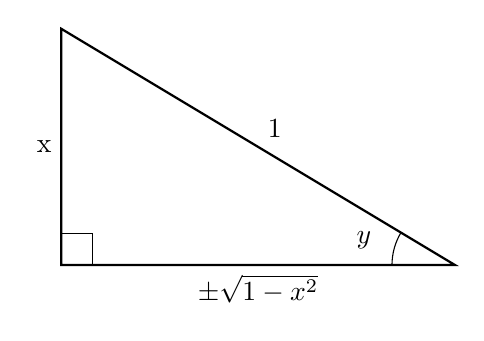
\begin{tikzpicture}
            \coordinate (A) at (0,3);
            \coordinate (B) at (5,0);
            \coordinate (C) at (0,0);
            \draw[thick] (A) -- (B) -- (C) -- cycle;
            
            \tkzLabelSegment[above right](A,B){1}
            \tkzLabelSegment[left](A,C){x}
            \tkzLabelSegment[below](B,C){$\pm \sqrt{1-x^2}$}

            \tkzMarkRightAngle[size=.4](A,C,B)
            \tkzMarkAngle[mark=none, size=0.8cm](A,B,C)
            \tkzLabelAngle[pos=1.2](A,B,C){$y$}
        \end{tikzpicture}
    \end{center}now with $a$ we can find $cos(y)$,
    \begin{center}
        \begin{align}
            cos(y)&=\frac{Adjacent}{Hypotenuse}\\
            cos(y)&=\pm \frac{\sqrt{1-x^2}}{1}\\
            \therefore cos(y)&=\pm \sqrt{1-x^2}
        \end{align}
    \end{center}
    because of the restriction of the values of $y$, the cosine of $y$ must be positive, thus,
    \begin{center}
        \begin{align}
            cos(y)&=\sqrt{1-x^2}\\
            \frac{dy}{dx} &=\frac{1}{\sqrt{1-x^2}}\\
            \therefore \frac{d}{dx}(sin^-(x)) &=\frac{1}{\sqrt{1-x^2}}
        \end{align}
    \end{center}
    this approach ended up the same answer to the problem. 
    
\newpage
\section{Implicit Differentiation of Inverses of Trigonometric Functions}

The final part of this article is to find $\frac{dy}{dx}$ of $sin^{-}( xy) =cos^{-}( x-y)$. To find $\frac{dy}{dx}$, we need to differentiate both side and isolate $\frac{dy}{dx}$, the derivative of $sin^-(x)$ is found at \eqref{eq:dasin}, to find the derivative of $cos^-(x)$, we follow the similar steps.

    \subsection{Derivative of Inverse Cosine Function}
    $\displaystyle \frac{d}{dx}\left( cos^{-}( x)\right)$ is equivalent to $\displaystyle \frac{dy}{dx}$ of the equation $\displaystyle \ y\ =cos^{-}( x)$, x is the independent variable and y is t he dependent variable,
     \begin{align}
        \label{yisarccosin}
        \ y\ &=cos^{-}( x)\\
        cos( y) &=cos\left( cos^{-}( x)\right)
    \end{align}
    using the inverse functions theorem $\displaystyle f\left( f^{-}( x)\right) =x$,
    \begin{align}
        \label{eq:cosy}
        cos(y)=x
    \end{align}
    differentiate both sides using the identity $\displaystyle cos'( x) =-sin( x) \times ( x) '$.%, and the chain rule $(x^n)^{'} = n x^{n-1} (x)^{'}$,
     \begin{align}
        ( cos( y))^{'} &=( x)^{'}\\
        -sin( y) \times \frac{dy}{dx} &=1\\
        \frac{dy}{dx} &=-\frac{1}{sin( y)}
    \end{align}
    we must change $sin(y)$ in terms of $x$ instead of $y$ since $y$ is the dependent variable and $x$ is the independent variable.

    Using the Pythagorean Identity derived previously,
    \begin{center}
        \begin{align}
            cos^2(\theta)+sin^2(\theta)&=1\\
            sin^2(\theta)&=1-cos^2(\theta)\\
            sin(\theta)&=\pm\sqrt{1-cos^2(\theta)}
        \end{align}
    \end{center}
    thus, the general form of $sin(\theta)$ is $\pm\sqrt{1-cos^2(\theta)}$.
    
    When changing $\theta$ to $y$, there are some restrictions. As shown in Section \ref{sec:arccosine}, the range of $arccos(x)$, or $cos^-(x)$ is $R: \{arccos(x)\in\mathbb{R}\:|\:arccos(x)\in [0, \pi]\}$. At 
    \eqref{yisarccosin} we found that $y$ is the arccosine of x, which means the range of $y$ is $R: \{y\in\mathbb{R}\:|\:y\in [0, \pi]\}$.
    
    By looking at the unit circle,
    \begin{center}
        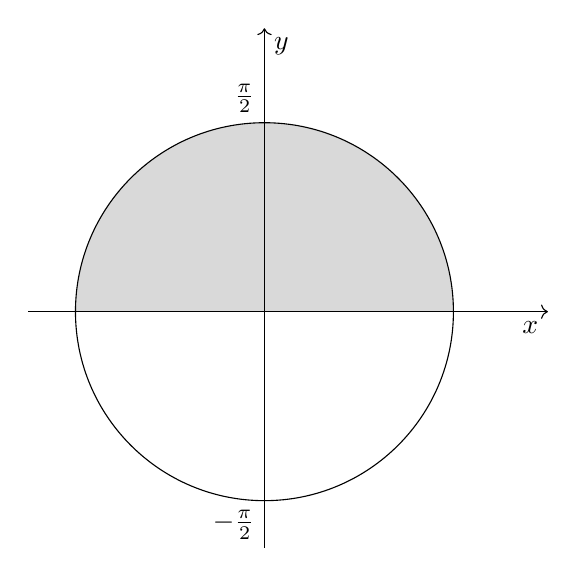
\begin{tikzpicture}[scale=2.4]
            \fill[gray!30] (0,0) -- (1,0) arc (0:180:1);
            \draw[->] (-1.25,0) -- (1.5,0) node[below left] {$x$};
            \draw[->] (0,-1.25) -- (0,1.5) node[below right] {$y$};
            \draw (0,0) circle [radius=1]; 
            \coordinate[label=above left:$\frac{\pi}{2}$] (Q) at (0,1);
            \coordinate[label=below left:$-\frac{\pi}{2}$] (P) at (0,-1);
        \end{tikzpicture}
    \end{center}

    as proved in Section \ref{sec:4.2}, for any point $P$ on the unit circle, the coordinate of $P$ is $cos(x), sin(x)$, thus within $y$'s range, the $y$ value must $\geq0$, or in other words, $sin(x)$ always $\geq0$.
    
    Also, as derived at \eqref{eq:cosy}, we can substitute $x$ to $cos(y)$.

    Therefore, we can convert $sin(y)$ to $\sqrt{1-x^2}$.

    Substituting $\sqrt{1-x^2}$ into $sin(y)$, we get:
    \begin{center}
        \begin{equation}
            \frac{dy}{dx} =-\frac{1}{\sqrt{1-x^2}}
        \end{equation}
    \end{center}
    converting back, 
    \begin{center}
        \begin{equation}
            \label{eq:dacos}
            \frac{d}{dx}(cos^-(x)) =-\frac{1}{\sqrt{1-x^2}}
        \end{equation}
    \end{center}

    \subsection{Solving the Implicit Differentiation}
    Now with the 2 derivatives derived at \eqref{eq:dasin} and at \eqref{eq:dacos}, we differentiate $sin^{-}( xy) =cos^{-}( x-y)$ and isolate $\frac{dy}{dx}$. Also, when differentiating a function, we must multiply the derivative of the argument, which needs to apply the product rule to separate $\frac{dy}{dx}$ from $\frac{d(xy)}{dx}$.

    \begin{equation}
        \centering
            sin^{-}( xy) =cos^{-}( x-y)
    \end{equation}
    
    First we can find the derivative of the left side of the equation, 
    \begin{align}
        \centering
        \frac{d}{dx}\left( sin^{-}( xy)\right) &=\frac{1}{\sqrt{1-( xy)^{2}}} \times \frac{d}{dx}( xy)\\
        \frac{d}{dx}\left( sin^{-}( xy)\right) &=\frac{1}{\sqrt{1-( xy)^{2}}} \times \left(\left(\frac{dx}{dx}\right) y+\left(\frac{dy}{dx}\right) x\right)\\
        \frac{d}{dx}\left( sin^{-}( xy)\right) &=\frac{y+\left(\frac{dy}{dx}\right) x}{\sqrt{1-( xy)^{2}}}
    \end{align}
    then we can find the derivative of the right side of the equation,
    \begin{align}
        \centering
        \frac{d}{dx}\left( cos^{-}( x-y)\right) &=-\frac{1}{\sqrt{1-( x-y)^{2}}} \times \frac{d}{dx}( x-y)\\
            \frac{d}{dx}\left( cos^{-}( x-y)\right) &=-\frac{1}{\sqrt{1-( x-y)^{2}}} \times \left(\frac{dx}{dx} -\frac{dy}{dx}\right)\\
            \frac{d}{dx}\left( cos^{-}( x-y)\right) &=-\frac{\left( 1-\frac{dy}{dx}\right)}{\sqrt{1-( x-y)^{2}}}
    \end{align}
    now substituting both sides into the equation, and isolate $\frac{dy}{dx}$,
    \begin{align}
    \centering
        \frac{y+\left(\frac{dy}{dx}\right) x}{\sqrt{1-( xy)^{2}}} &=-\frac{\left( 1-\frac{dy}{dx}\right)}{\sqrt{1-( x-y)^{2}}}\\
        \left( y+\left(\frac{dy}{dx}\right) x\right)\sqrt{1-( x-y)^{2}} &=-\left( 1-\frac{dy}{dx}\right)\sqrt{1-( xy)^{2}}\\
        y\sqrt{1-( x-y)^{2}} +\sqrt{1-( xy)^{2}} &=\frac{dy}{dx}\left(\sqrt{1-( xy)^{2}} -x\sqrt{1-( x-y)^{2}}\right)
    \end{align}
    here is the final equation derived,
    \begin{equation}
        \therefore \frac{dy}{dx} =\frac{y\sqrt{1-( x-y)^{2}} +\sqrt{1-( xy)^{2}}}{\sqrt{1-( xy)^{2}} -x\sqrt{1-( x-y)^{2}}}
    \end{equation}

    There are several ways to derive the final equation for $\frac{dy}{dx}$ of the equation $arcsin(xy)=arccos(x-y)$, only one way is shown above, but we can also use the identity that $cos(arcsin(xy))=\pm\sqrt{1-(xy)^2}$ to change the equation to $x-y=\pm\sqrt{1-(xy)^2}$ which can be proved using the Pythagorean Theorem and the definition of sine, cosine, then differentiate and get a simpler answer; or we can also use the identity that $sin(arccos(x-y))=\pm\sqrt{1-(x-y)^2}$ which can be proved as above. 

    Because of the complexity of this equation, it is very hard to find all restrictions for x and y values. Furthermore, because of the derivative of the equation has 2 independent variables, we can say that this is a binary function, thus 3-dimensional plot is require, which without any original restrictions can be shown as:\\
    
    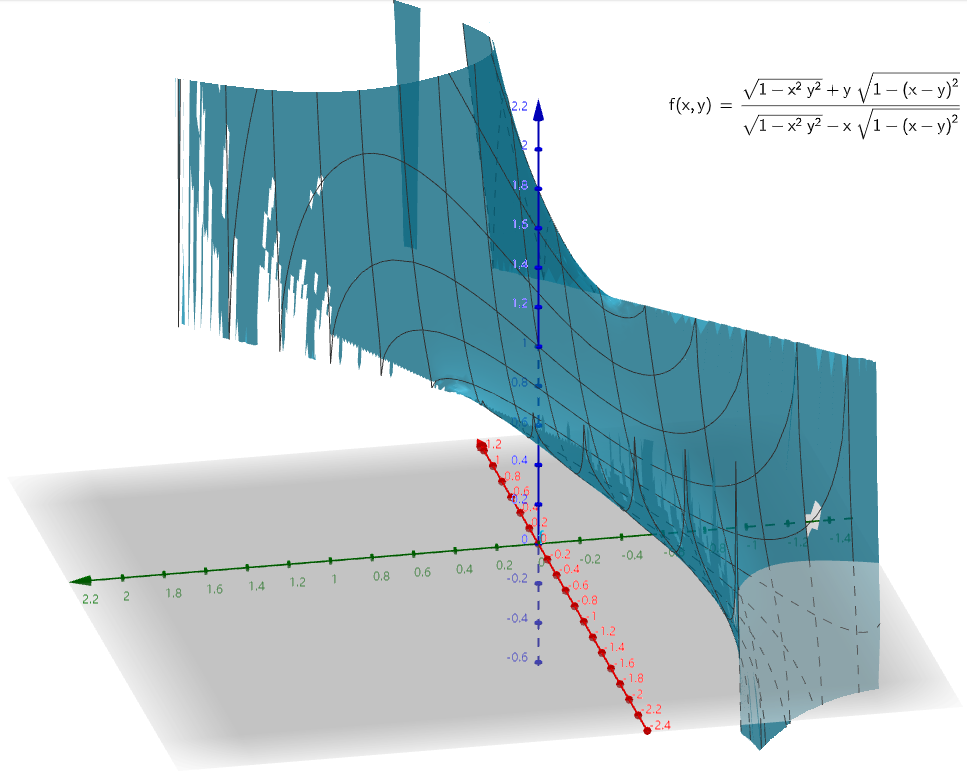
\includegraphics[scale=0.51]{1111}

    \section{Conclusion}
    In conclusion, 
    \begin{enumerate}
        \item The graph of the unrestricted inverse $f^-$ can be found by reflecting the original unrestricted function $f$ along the line $y=x$.
        \item The domain of the unrestricted function $f$ is the range of its unrestricted inverse $f^-$; the range of the unrestricted function $f$ is the domain of its unrestricted inverse $f^-$.
        \item Let $f(x)$ be any function, to find the equation for the inverse $f^-(x)$, we can first exchange the positions of $f(x)$ and $x$, and change $f(x)$ to $f^-(x)$, then isolate $f^-(x)$ and get the equation of $f^-(x)$.
        \item All horizontal asymptotes of the function $f$ become the vertical asymptotes of its inverse $f^-$;  all vertical asymptotes of the function $f$ become the horizontal asymptotes of its inverse $f^-$ which in both cases $f$ and $f^-$ are not restricted.
        \item To avoid relation, we restrict the inverse of trigonometric functions.
        \item If $f$ and $f^-$ are 2 functions such that $f(f^-(x)) = x$ for every $x$ in the domain of $f^-$, and, $f^-(f(x)) = x$, for every $x$ in the domain of $f$, then $f$ and $f^-$ are inverse functions of each other. 
        \item A function $f$ has an inverse function $f^-$ if and only if the function $f$ passes the horizontal line test, which means no horizontal line intersects its graph more than once.
        \item If $f$ is either always increasing or decreasing in an interval, then $f$ has an inverse.
        \item If $f$ is differentiable at every point on an interval, and $f'(x)\neq0$ on this interval, then the inverse $f^-$ is differentiable at every point within the interval and $(f^-(x))'=\frac{1}{f'(f^-(x))}$ (In other words, the derivative of the inverse $f^-(x)$ at $x=a$ is equal to the reciprocal of the derivative of the original function $f(x)$ which takes $f^-(x), x=a$ as the argument because of the property of inverse functions).
    \end{enumerate}

    By looking at the first graph at Section \ref{sec:simp}, we can see that the derivative of the inverse is the reciprocal of the original function, but further prove need to be shown. Here is the prove of the last conclusion:
    
    Let $x$ be the independent variable and $y$ be the inverse of the function $f(x)$ which is $f^-(x)$, since $f(f^-(x))=x$, thus $f(y)=x$, now we differentiate both sides with respect to x,
    \begin{align}
        \centering
        f(y)&=x\\
        f'(y)\times\frac{dy}{dx}&=1\\
        \frac{dy}{dx}&=\frac{1}{f'(y)}
    \end{align}
    changing $y$ back to $f^-(x)$ we get,
    \begin{align}
        \centering
        \frac{d}{dx}(f^-(x))&=\frac{1}{f'(f^-(x))}\\
        (f^-(x))'&=\frac{1}{f'(f^-(x))}
    \end{align}
    therefore this property is proved.
\end{document}